\ifx\wholebook\relax \else

\documentclass[b5paper]{ctexart}
\usepackage[nomarginpar
  %, margin=.5in
]{geometry}

\addtolength{\oddsidemargin}{-0.05in}
\addtolength{\evensidemargin}{-0.05in}
\addtolength{\textwidth}{0.1in}

\usepackage[cn]{../../../prelude}

\setcounter{page}{1}

\begin{document}

\title{二叉搜索树}

\author{刘新宇
\thanks{{\bfseries 刘新宇} \newline
  Email: liuxinyu95@gmail.com \newline}
  }

\maketitle
\fi

\markboth{二叉搜索树}{基本算法}

\ifx\wholebook\relax
\chapter{二叉搜索树}
\numberwithin{Exercise}{chapter}
\fi

数组和链表通常被认为是最基础的数据结构,其实它们并不简单(第12章)。在某些系统中,数组是最基本的组件,甚至链表也可以由数组来实现(\cref{sec:list-index-array})。另一方面,在函数式环境中,链表被作为最基本的组件来实现数组和其它更复杂的数据结构。二叉搜索树是另一种基础数据结构。乔$\cdot$本特利在《编程珠玑》\cite{Bentley}中,讨论了如何统计一段文字中各单词的个数。下面的例子程序给出了一个解法。\index{统计单词}

\lstset{frame=single}
\begin{lstlisting}[language=Bourbaki]
void wordCount(Input in) {
    Map<String, Int> map
    while String w = read(in) {
        map[w] = if map[w] == null then 1 else map[w] + 1
    }
    for var (w, c) in map {
        print(w, ":", c)
    }
}
\end{lstlisting}

%% 我们可以运行下面的命令进行统计:

%% \begin{verbatim}
%% $ cat bbe.txt | wordcount > wc.txt
%% \end{verbatim}

\section{定义}
\label{introduction} \index{二叉树}

这里的\texttt{map}是用二叉搜索树实现的字典数据结构。我们用单词作为键,用单词出现的次数作为值。这段程序展示了二叉搜索树的典型应用。我们先了解一下二叉树。一棵二叉树或者为空($\nil$)\footnote{$\nil$是数学家安德烈$\cdot$韦伊引入的挪威语字母,用来表示空集。},或者包含三个部分:一个元素$k$和左右两个分支$l$、$r$,这两个分支也都是二叉树,记为$(l, k, r)$。左右分支也被称为左子树和右子树,或统称为孩子。也可以说一棵树由若干节点构成。节点或为空或包含类型为$K$的值。二叉树的类型为$Tree\ K$。如果一个节点的左右子树都为空,我们称之为叶子节点,否则称为分支节点。

\begin{figure}[htbp]
  \centering
  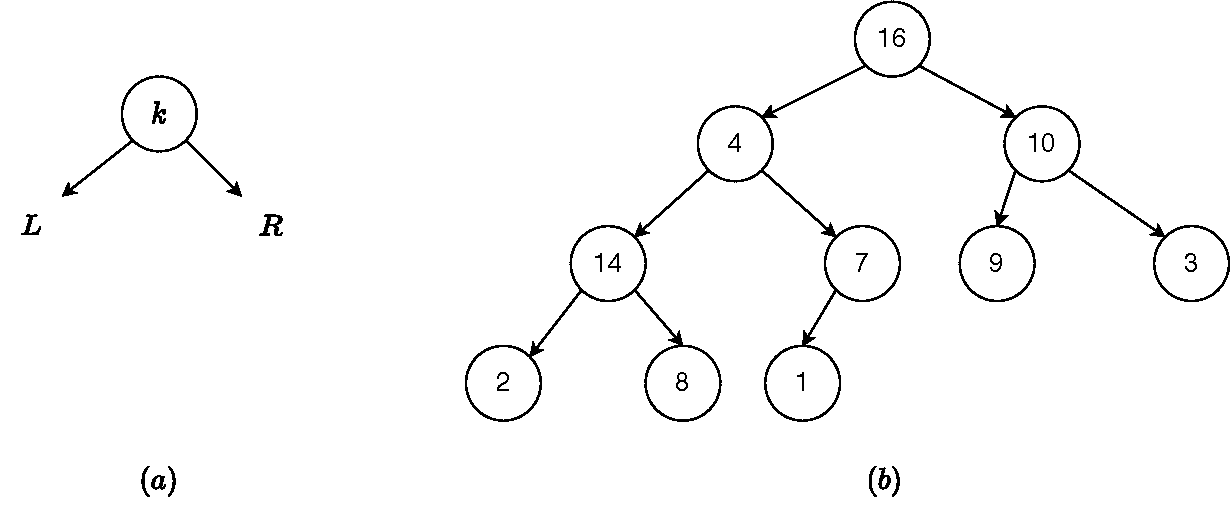
\includegraphics[scale=0.6]{img/binary-tree}
  \caption{二叉树的结构和例子}
  \label{fig:binary-tree-example}
\end{figure}

\index{二叉搜索树}
二叉搜索树是一种特殊的二叉树,它的值可以进行比较\footnote{广义比较,例如大小,先后、包含等序关系。本章中的“小于”及其符号$<$是抽象的比较。},并且满足:对于任何非空节点$(l, k, r)$,左侧分支中所有的值都小于$k$;$k$小于右侧分支中所有的值。\cref{fig:bst-example}展示了一棵二叉搜索树。和\cref{fig:binary-tree-example}比较,可以看到节点组织方式的不同。一棵二叉树的值可以是任意类型,而二叉搜索树要求它的值必须能进行比较\footnote{只要能进行抽象的“小于”和“等于”比较就足够了。}。为了强调这种区别,我们特别称二叉搜索树的值为键(key),称节点中存储的其它数据为值(value),其类型为$Tree\ (K, V)$。为了方便上溯到祖先,可以在节点中存储父节点引用。我们在上下文清楚的情况下忽略值。本章附录给出了例子定义。在函数式环境中,一般不使用引用或指针回溯,而用自顶向下的递归进行计算。下面是函数式定义的例子(这类定义称为代数数据类型,简写为ADT):

\begin{figure}[htbp]
  \centering
  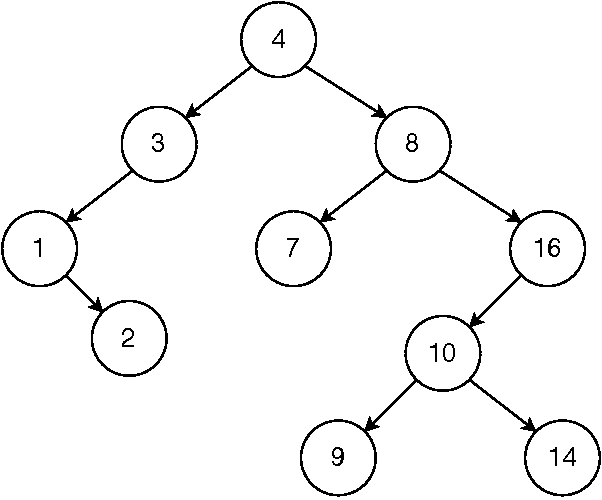
\includegraphics[scale=0.5]{img/bst-example}
  \caption{二叉搜索树的例子} \label{fig:bst-example}
\end{figure}

\begin{Haskell}
data Tree a = Empty | Node (Tree a) a (Tree a)
\end{Haskell}

\section{插入}
\index{二叉搜索树!插入}

向二叉搜索树插入$k$(和相关的数据)时,需要确保树中元素有序。插入操作定义如下:(1)如果树为空,创建一个元素为$k$的叶子节点;(2)如果$k$小于根节点中的元素,将它插入到左子树中;否则,将$k$插入到右子树中。当$k$等于根节点中的元素时,说明它已经存在了。我们可以覆盖掉以前的数据(更新),或把新数据添加在后面,也可以跳过不做处理。简单起见,我们忽略这一情况。

\be
\begin{array}{rcl}
insert\ k\ \nil & = & (\nil, k, \nil) \\
insert\ k\ (l, x, r) & = & \begin{cases}
  k < x: & (insert\ k\ l, x, r) \\
  \text{否则}: & (l, x, insert\ k\ r) \\
  \end{cases}
\end{array}
\ee

下面是相应的例子程序:

\begin{Haskell}
insert k Empty = Node Empty k Empty
insert k (Node l x r) | k < x = Node (insert k l) x r
                      | otherwise = Node l x (insert k r)
\end{Haskell}

这一例子程序使用了模式匹配。本章附录给出了不使用此特性的例子。也可以消除递归,用迭代实现插入:

\begin{algorithmic}[1]
\Function{Insert}{$T, k$}
  \State $root \gets T$
  \State $x \gets$ \Call{Create-Leaf}{$k$}
  \State $parent \gets$ NIL
  \While{$T \neq$ NIL}
    \State $parent \gets T$
    \If{$k <$ \Call{Key}{$T$}}
      \State $T \gets $ \Call{Left}{$T$}
    \Else
      \State $T \gets $ \Call{Right}{$T$}
    \EndIf
  \EndWhile
  \State \Call{Parent}{$x$} $\gets parent$
  \If{$parent = $ NIL} \Comment{$T$为空}
    \State \Return $x$
  \ElsIf{$k <$ \Call{Key}{$parent$}}
    \State \Call{Left}{$parent$} $\gets x$
  \Else
    \State \Call{Right}{$parent$} $\gets x$
  \EndIf
  \State \Return $root$
\EndFunction
\Statex
\Function{Create-Leaf}{k}
  \State $x \gets $ \Call{Empty-Node}{}
  \State \Call{Key}{$x$} $ \gets k$
  \State \Call{Left}{$x$} $ \gets $ NIL
  \State \Call{Right}{$x$} $ \gets $ NIL
  \State \Call{Parent}{$x$} $ \gets $ NIL
  \State \Return $x$
\EndFunction
\end{algorithmic}

其中\textproc{Key}($T$)获取二叉树节点中的值,它可以定如下:

\be
\begin{array}{rcl}
key\ \nil & = & \textit{Nothing} \\
key\ (l, k, r) & = & \textit{Just}\ k \\
\end{array}
\ee

我们可以连续插入,将一组元素转变成二叉搜索树:

\[
\begin{array}{rcl}
\textit{fromList}\ [\ ] & = & \nil \\
\textit{fromList}\ (x \cons xs) & = & insert\ x\ (\textit{fromList}\ xs) \\
\end{array}
\]

或通过叠加(第1章)将\textit{fromList}定义为(柯里化):\textit{fromList} = $foldr\ insert\ \nil$。我们特意将参数顺序设计为对称的$insert\ k\ t$和\textproc{Insert}($T, k$)。前者用$foldr$,后者用$foldl$(或for循环):

\begin{algorithmic}[1]
\Function{From-List}{$X$}
  \State $T \gets $ NIL
  \For{each $x$ in $X$}
    \State $T \gets$ \Call{Insert}{$T, x$}
  \EndFor
  \State \Return $T$
\EndFunction
\end{algorithmic}

\section{遍历}
\index{二叉树!遍历}

遍历是指依次访问二叉树中的每个元素。有三种遍历方法:前序遍历、中序遍历、后序遍历。它们是按照访问根节点和子节点的先后顺序命名的。

\begin{itemize}
\item 前序遍历:先访问\textbf{根节点},然后访问左子树,最后访问右子树;
\item 中序遍历:先访问左子树,然后访问\textbf{根节点},最后访问右子树;
\item 后序遍历:先访问左子树,然后访问右子树,最后访问\textbf{根节点}。
\end{itemize}

\index{前序遍历} \index{中序遍历} \index{后序遍历}

所有的“访问”操作都是递归的。\textbf{先}访问根后访问子分支称为\textbf{先序},在访问左右分支的\textbf{中间}访问根称为\textbf{中序},先访问子分支\textbf{后}访问根称为\textbf{后序}。对于\cref{fig:bst-example}中的二叉树,三种遍历的结果分别如下:

\begin{itemize}
\item 前序遍历:4, 3, 1, 2, 8, 7, 16, 10, 9, 14
\item 中序遍历:1, 2, 3, 4, 7, 8, 9, 10, 14, 16
\item 后序遍历:2, 1, 3, 7, 9, 14, 10, 16, 8, 4
\end{itemize}

特别地,中序遍历会按照从小到大的顺序输出元素。二叉搜索树的定义保证了这一性质(\cref{ex:BST-in-order-sort})。定义$map$按中序遍历顺序将函数$f$应用到每个元素上,从而映射成另一棵同构的树。

\be
\begin{array}{rcl}
map\ f\ \nil & = & \nil \\
map\ f\ (l, k, r) & = & (map\ f\ l, f\ k, map\ f\ r)
\end{array}
\ee

如果只访问、操作各节点的值,无需创建另外一棵树,我们可以实现如下的中序遍历:

\begin{algorithmic}[1]
\Function{Traverse}{$T, f$}
  \If{$T \neq$ NIL}
    \State \textproc{Traverse}(\Call{Left}{$T$}, $f$)
    \State $f$(\Call{Key}{$T$})
    \State \textproc{Traverse}(\Call{Right}{$T$, $f$})
  \EndIf
\EndFunction
\end{algorithmic}

我们可以修改$map$,通过中序遍历将一棵二叉搜索树转化为有序序列:

\be
\begin{array}{rcl}
toList\ \nil & = & [\ ] \\
toList\ (l, k, r) & = & toList\ l \doubleplus [k] \doubleplus toList\ r \\
\end{array}
\ee

据此可以得到一个排序方法:先把无序列表转化为二叉搜索树,再用中序遍历把树转换回有序列表。称为“树排序”:$sort\ X = toList\ (\textit{fromList}\ X)$,或写成函数组合\cite{func-composition}的形式:

\be
  sort = toList \circ \textit{fromList}
\ee

我们可以对二叉树进行中序叠加(叠加的概念见第一章)。

\be
\begin{array}{rcl}
foldt\ f\ g\ z\ \nil & = & z \\
foldt\ f\ g\ z\ (l, k, r) & = & g\ (foldt\ f\ g\ z\ l)\ (f\ k)\ (foldt\ f\ g\ z\ r) \\
\end{array}
\ee

这里$f: A \to B$,将树中类型为$A$的元素映射为$B$,这样$f(k) = m$。它递归地对左右子树叠加(从$z$开始)得到$x$和$y$,然后用$g$将三个值组合起来$g\ x\ m\ y$。利用$foldt$,我们可以定义二叉树的映射$map$为:

\be
map\ f = foldt\ f\ (x\ m\ y\ \mapsto (x, m, y))\ \nil
\ee

$foldt$在叠加时利用三元函数$g$保存了二叉树的结构,如果不关心结构,可以利用二元函数$f : A \times B \to B$实现叠加,将类型为$Tree\ A$的树叠加为类型为$B$的值:

\be
\begin{array}{rcl}
fold\ f\ z\ \nil & = & z \\
fold\ f\ z\ (l, k, r) & = & fold\ f\ (f\ k\ (fold\ f\ z\ r))\ l\\
\end{array}
\ee

例如:$sum = fold\ (+)\ 0$将二叉树中所有的元素累加起来。$length = fold\ (x\ n \mapsto n + 1)\ 0$可以统计树中元素个数。但是$fold$无法定义$map$,因为二元函数$f$丢失了树结构。

\begin{Exercise}\label{ex:bst-traverse}
\index{重建树}
\Question{给定如下前序遍历和中序遍历的结果,请重建出二叉树,并给出后序遍历的结果。
  \begin{itemize}
  \item 前序遍历结果:1, 2, 4, 3, 5, 6
  \item 中序遍历结果:4, 2, 1, 5, 3, 6
  \item 后序遍历结果:?
  \end{itemize}
}

\Question{编程实现从前序遍历和中序遍历的结果重建二叉树。}

\Question{证明对二叉搜索树进行中序遍历可以将全部元素按照从小到大的顺序输出。
\label{ex:BST-in-order-sort}
}

\Question{对于$n$个元素,树排序的算法复杂度是什么?}

\Question{使用叠加定义$toList$}

\Question{使用叠加定义$depth\ t$,获得一棵二叉树的高度。}
\end{Exercise}

\begin{Answer}[ref={ex:bst-traverse}]
\Question{给定如下前序遍历和中序遍历的结果,请重建出二叉树,并给出后序遍历的结果。
\begin{itemize}
\item 前序遍历结果:1, 2, 4, 3, 5, 6
\item 中序遍历结果:4, 2, 1, 5, 3, 6
\item 后序遍历结果:?
\end{itemize}

[4, 2, 5, 6, 3, 1]
}

\Question{编程实现从前序遍历和中序遍历的结果重建二叉树。

\vspace{3mm}
记前序遍历结果为$P$,中序遍历结果为$I$。如果$P = I = [\ ]$,则二叉树为空$\nil$。否则,前序遍历是递归的“根、左、右”,因此$P$中第一个元素$m$是根节点的值。中序遍历是递归的“左、根、右”,我们一定可以在$I$中找到$m$,并把$I$分成三部分:$[a_1, a_2, ..., a_{i-1}, m, a_{i+1}, a_{a+2}, ..., a_n]$,令:$I_l = I[1, i), I_r = I[i+1, n]$,其中$[l, r)$表示左闭右开区间,包括$l$但不包括$r$,它们可以为空$[\ ]$。这三部分$I_l, m, I_r$中,$I_l$是左子树的中序遍历结果,$I_r$是右子树的中序遍历结果。令$k = |I_l|$表示左子树的大小,我们可以用$k$分割$P[2, n]$为两部分:$P_l, P_r$,其中$P_l$是前$k$个元素,$P_r$是剩余部分。这样我们就可以递归地用$(P_l, I_l)$重建左子树,用$(P_r, I_r)$重建右子树:

\[
\begin{array}{rcl}
\textit{rebuild}\ [\ ]\ [\ ] & = & \nil \\
\textit{rebuild}\ (m \cons ps)\ I & = & (\textit{rebuild}\ P_l\ I_l, m, \textit{rebuild}\ P_r\ I_r) \\
\end{array}
\]
其中:

\[
\begin{cases}
(I_l, I_r) & = \textit{splitWith}\ m\ I \\
(P_l, P_r) & = \textit{splitAt}\ |I_l|\ ps \\
\end{cases}
\]

下面是例子程序:
\begin{Haskell}
rebuild [] _ = Empty
rebuild [c] _ = Node Empty c Empty
rebuild (x:xs) ins = Node (rebuild prl inl) x (rebuild prr inr) where
  (inl, _:inr) = (takeWhile (/= x) ins, dropWhile (/=x) ins)
  (prl, prr) = splitAt (length inl) xs
\end{Haskell}

也可以通过更新左右边界来实现:
\begin{lstlisting}[language = Bourbaki]
Node<T> rebuild([T] pre, [T] ins, Int l = 0, Int r = length(ins)) {
    if l >= r then return null
    T c = popFront(pre)
    Int m = find(c, ins)
    var left = rebuild(pre, ins, l, m)
    var right = rebuild(pre, ins, m + 1, r)
    return Node(left, c, right)
}
\end{lstlisting}
}

\Question{证明对二叉搜索树进行中序遍历可以将全部元素按照从小到大的顺序输出。
\begin{proof}
使用反证法。假设存在二叉搜索树,其中序遍历结果无序。我们在所有中序遍历无序的树中,选出一棵最小的$T$。首先$T$不可能为空$\nil$, 空树的中序遍历结果为$[\ ]$是有序的。其次$T$不可能是叶子$T = (\nil, k, \nil)$,叶子的中序遍历结果为$[k]$是有序的。因此$T$只能是分枝节点$(l, k, r)$,中序遍历结果为$toList\ l \doubleplus [x] \doubleplus toList\ r$。由于$T$是最小的中序遍历无序的树,而$l$、$r$都比$T$小,所以$toList\ l$和$toList\ r$都有序。根据二叉搜索树的定义,任何$x \in l, x < k$,任何$y \in r, y > k$。所以中序遍历结果$toList\ l \doubleplus [x] \doubleplus toList\ r$有序。这与假设$T$的中序遍历结果无序矛盾。所以任何二叉搜索树的中序遍历结果有序。
\end{proof}
}

\Question{对于$n$个元素,树排序的算法复杂度是什么?

$(n \lg n)$
}

\Question{使用叠加定义$toList$
\[
\begin{array}{rcl}
toList & = & foldt\ id\ (as\ b\ bs \mapsto as \doubleplus b : bs)\ [\ ] \\
       & = & fold\ (:)\ [\ ] \\
\end{array}
\]
}

\Question{使用叠加定义$depth\ t$,获得一棵二叉树的高度。\label{ex:bst-depth}
\[
depth = foldt\ (x \mapsto 1)\ (x\ d\ y\ \mapsto d + \max\ x\ y)\ 0
\]
}
\end{Answer}

\section{查找}
\index{二叉搜索树!查找}

由于二叉搜索树中的元素是按序递归存储的,它可以方便地支持各种搜索。这也是人们将其命名为“搜索树”的原因。有三种不同类型的搜索:1)在树中查找一个键;2)寻找最大或最小元素;3)查找某一元素的前驱(上一个)或后继(下一个)元素。考虑在类型为$Tree\ (K, V)$的二叉搜索树中查找某个键$x$对应的值:

\begin{itemize}
\item 如果树为空,$x$不存在;
\item 如果根节点元素$(k, v)$中$k = x$,结果为$v$;
\item 如果$x < k$,在左子树中递归查找;否则在右子树中递归查找。
\end{itemize}

\be
\begin{array}{rcl}
lookup\ x\ \nil & = & \textit{Nothing} \\
lookup\ x\ (l, (k, v), r), x) & = & \begin{cases}
  k = x: & \textit{Just}\ v \\
  x < k: & lookup\ x\ l \\
  \text{否则}: & lookup\ x\ r \\
  \end{cases}
\end{array}
\ee

这里使用$Maybe$类型\footnote{也叫作\texttt{Optional<T>}类型,见第一章。}处理未找到的情况。如果二叉树平衡(见第四章),对于$n$个元素的二叉树,查找的性能为$O(\lg n)$。如果二叉树很不平衡,查找的时间在最坏情况下退化到$O(n)$。如果记树的高度为$h$,则查找算法的性能可以表示成$O(h)$的形式。下面是消除递归的迭代式实现:

\begin{algorithmic}[1]
\Function{Lookup}{$T, x$}
  \While{$T \neq $ NIL 且 \Call{Key}{$T$} $ \neq x$}
    \If{$x <$ \Call{Key}{$T$}}
      \State $T \gets $ \Call{Left}{$T$}
    \Else
      \State $T \gets $ \Call{Right}{$T$}
    \EndIf
  \EndWhile
  \State \Return \Call{Value}{$T$}  \Comment{$T = $NIL返回$\nil$}
\EndFunction
\end{algorithmic}

\index{二叉搜索树!最小元素/最大元素}
在二叉搜索树中,较小的元素总是位于左侧分支,而较大的元素总是位于右侧分支。可以利用这一特性来定位最大、最小元素。为了找到最小元素,我们可以不断向左侧前进,直到左侧分支为空。对称地,我们可以通过不断向右侧前进找到最大元素。这两个函数的性能都是$O(h)$,其中$h$是树的高度。

\be
\begin{array}{cc}
  \begin{array}{rcl}
  \min\ (\nil, k, r) & = & k \\
  \min\ (l, k, r) & = & \min\ l \\
  \end{array}
&
  \begin{array}{rcl}
  \max\ (l, k, \nil) & = & k \\
  \max\ (l, k, r) & = & \max\ r \\
  \end{array}
\end{array}
\ee

\index{二叉搜索树!前驱/后继}
有时需要把二叉搜索树当作容器遍历。例如从最小的元素开始,逐一向前移动到最大元素,或者按需先后移动。下面的例子程序升序输出树中的元素:

\lstset{language=Bourbaki}
\begin{lstlisting}
void printTree (Node<T> t) {
    for var it = Iterator(t), it.hasNext(), it = it.next() {
        print(it.get(), ", ")
    }
}
\end{lstlisting}

这需要查找一个节点的前驱或后继元素。$x$的后继定义为满足$x < y$的最小$y$。如果$x$的右子树不为空,则右子树中的最小值就是后继。\cref{fig:bst-succ}中8的后继元素为9,它是8的右子树中的最小值。如果$x$的右子树为空,需要向上回溯,找到最近的一个祖先$p$,使得$p$的左子树也是$x$的祖先。在\cref{fig:bst-succ}中,元素2所在的节点没有右侧分支,向上回溯一步到元素1,但是1没有左侧分支,继续向上查找到元素3。3的左子树也是2的祖先。这样2的后继为3。

\begin{figure}[htbp]
  \centering
  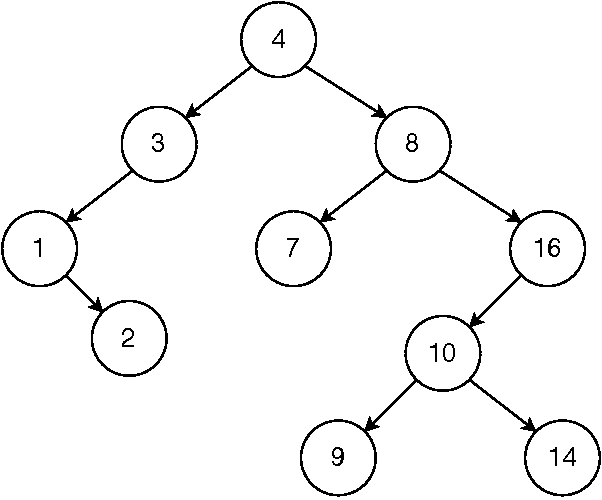
\includegraphics[scale=0.5]{img/bst-example}
  \caption{8的后继为其右侧分支的最小值9;为了获得2的后继,首先向上找到1,它没有左子树,继续向上找到3,3的左子树也是2的祖先,故而后继为3。} \label{fig:bst-succ}
\end{figure}

如果沿着父节点引用一直回溯到了根节点,仍然没有找到位于右侧的祖先,这说明$x$没有后继(树中最后一个元素)。

\begin{algorithmic}[1]
\Function{Succ}{$x$}
  \If{\Call{Right}{$x$} $\neq $ NIL}
    \State \Return \textproc{Min}(\Call{Right}{$x$})
  \Else
    \State $p \gets $ \Call{Parent}{$x$}
    \While{$p \neq $ NIL 且 $x =$ \Call{Right}{$p$}}
      \State $x \gets p$
      \State $p \gets $ \Call{Parent}{$p$}
    \EndWhile
    \State \Return $p$
  \EndIf
\EndFunction
\end{algorithmic}

当$x$没有后继时返回NIL。寻找前驱元素与此对称:

\begin{algorithmic}[1]
\Function{Pred}{$x$}
  \If{\Call{Left}{$x$} $\neq $ NIL}
    \State \Return \textproc{Max}(\Call{Left}{$x$})
  \Else
    \State $p \gets $ \Call{Parent}{$x$}
    \While{$p \neq $ NIL 且 $x =$ \Call{Left}{$p$}}
      \State $x \gets p$
      \State $p \gets $ \Call{Parent}{$p$}
    \EndWhile
    \State \Return $p$
  \EndIf
\EndFunction
\end{algorithmic}

纯函数式环境中一般不使用父节点引用\footnote{ML或OCaml中有\texttt{ref}引用概念,这里我们限于纯函数式环境。}。有的实现在遍历时留下标记,用以将来回溯甚至重建整棵树,称为zipper(\cite{learn-haskell}最后一章)。查找前驱和后继的初衷是“作为一个通用容器,遍历树中的全部元素”。在纯函数式环境中,我们通常用$map$中序遍历所有元素。前驱和后续的查找,仅在命令式环境中才有意义。

\begin{Exercise}\label{ex:bst-lookup}
\Question{判断某个值$k$是否存在于类型为$Tree\ K$的二叉搜索树$t$中。}

\Question{使用\textproc{Pred}和\textproc{Succ}实现一个二叉搜索树的迭代器。用它遍历一棵含有$n$个元素的树的复杂度是什么?}\label{itm:bst-iterate}

\Question{下面程序可以遍历一个区间$[a, b]$内的元素:

\texttt{for\_each (m.lower\_bound(12), m.upper\_bound(26), f)}

试用纯函数式的方法解决这一问题
\index{区间遍历}
}
\end{Exercise}

\begin{Answer}[ref={ex:bst-lookup}]
\Question{判断某个值$k$是否存在于类型为$Tree\ K$的二叉搜索树$t$中。
\begin{Haskell}
member x (Node l k r) | x == k = True
             | x < k = member x l
             | otherwise = member x r
\end{Haskell}
}

\Question{使用\textproc{Pred}和\textproc{Succ}实现一个二叉搜索树的迭代器。用它遍历一棵含有$n$个元素的树的复杂度是什么?

\begin{Bourbaki}
data TreeIterator<T> {
    Node<T> node = null

    TreeIterator(Node<T> root) { node = min(root) }

    T get() = node.key

    Bool hasNext() = node != null

    Self next() { if hasNext() then node = succ(node) }
}
\end{Bourbaki}

尽管在访问前驱和后继元素时需要寻找子树的最大(小)值,或沿着父节点回溯,但使用迭代器遍历搜索树容器却只需要线性时间。在遍历时,对于每个节点,我们仅访问一次(到达一次、离开一次)。例如:

\begin{Bourbaki}
for var it = TreeIterator(root), it.hasNext(), it = it.next() {
    print(it.get())
}
\end{Bourbaki}
所以遍历的复杂度为$O(n)$。
}

\Question{下面程序可以遍历一个区间$[a, b]$内的元素:

\texttt{for\_each (m.lower\_bound(12), m.upper\_bound(26), f)}

试用纯函数式的方法解决这一问题

\begin{Haskell}
mapR f a b t = map' t where
    map' Empty = Empty
    map' (Node l k r) | k < a = map' r
                      | a <= k && k <= b = Node (map' l) (f k) (map' r)
                      | k > b = map' l
\end{Haskell}
}
\end{Answer}

\section{删除}
\index{二叉搜索树!删除}
我们必须保证删除后二叉搜索树仍保持有序:节点的左侧分支元素仍小于节点中元素,右侧分支元素仍大于节点中元素。直接删除节点会破坏这一性质。删除节点$x$的方法如下\cite{sgi-stl}:(1)如果$x$是叶子节点或只有一棵非空子树,直接将$x$“切掉”;(2)如果$x$有两棵非空子树,用右子树中的最小值$y$替换掉$x$,然后将原先的$y$“切掉”。我们利用了这样的特性:右子树中的最小值不可能有两棵非空子树。这样就把第二种情况转化为第一种,从而直接将原最小节点“切掉”。如同\cref{fig:del-leaf}、\cref{fig:del-1child}、\cref{fig:del-branch}所示。

\begin{figure}[htbp]
  \centering
  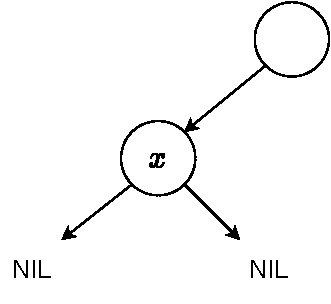
\includegraphics[scale=0.6]{img/del-leaf}
  \caption{直接“切掉”叶子节点$x$。}
  \label{fig:del-leaf}
\end{figure}

\begin{figure}[htbp]
  \centering
  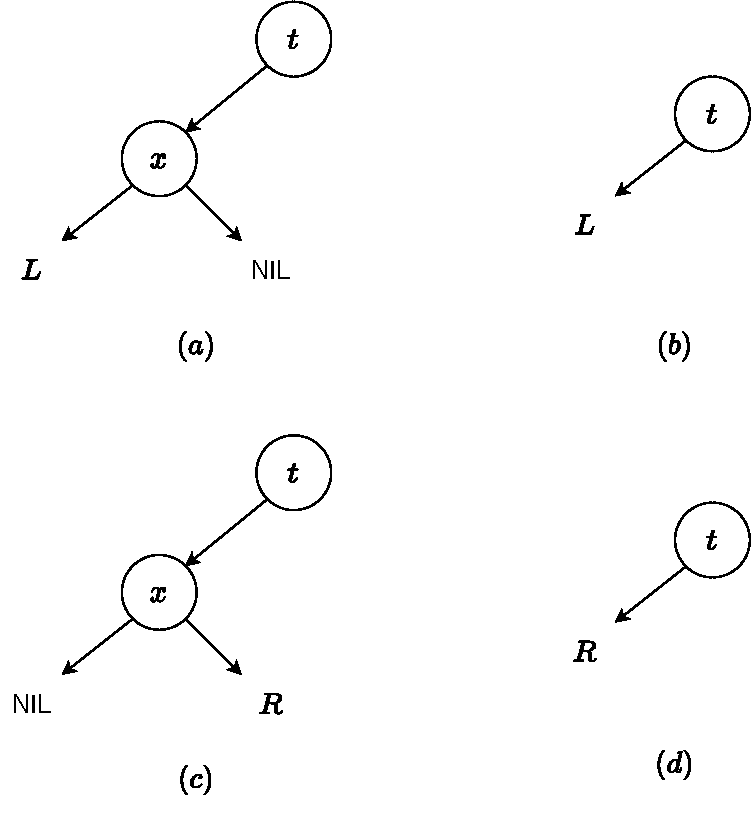
\includegraphics[scale=0.6]{img/del-singleton}
  \caption{删除只有一个非空分支的节点}
  \label{fig:del-1child}
\end{figure}

\begin{figure}[htbp]
  \centering
  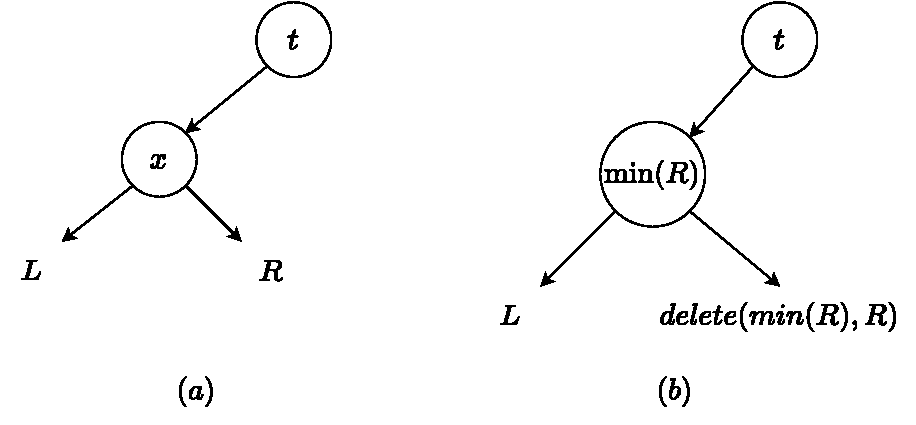
\includegraphics[scale=0.6]{img/del-branch}
  \caption{删除有两个非空分支的节点}
  \label{fig:del-branch}
\end{figure}

\be
\begin{array}{rcl}
delete\ x\ \nil & = & \nil\\
delete\ x\ (l, k, r) & = & \begin{cases}
  x < k: & (delete\ x l, k, r) \\
  x > k: & (l, k, delete\ x r) \\
  x = k: & del\ l\ r \\
\end{cases}
\end{array}
\ee

其中:

\be
\begin{array}{rcl}
del\ \nil\ r & = & r \\
del\ l\ \nil & = & l \\
del\ l\ r & = & (l, y, delete\ y\ r), y = \min\ r \\
\end{array}
\ee

删除算法的复杂度为$O(h)$,其中$h$是树的高度。命令式算法需要在删除后设置父节点。

\begin{algorithmic}[1]
\Function{Delete}{$T, x$}
  \State $r \gets T$
  \State $x' \gets x$ \Comment{保存$x$}
  \State $p \gets $ \Call{Parent}{$x$}
  \If{\Call{Left}{$x$} $= $ NIL}
    \State $x \gets $ \Call{Right}{$x$}
  \ElsIf{\Call{Right}{$x$} $= $ NIL}
    \State $x \gets $ \Call{Left}{$x$}
  \Else
    \Comment{两个分支都不为空}
    \State  $y \gets $ \textproc{Min}(\Call{Right}{$x$})
    \State \Call{Key}{$x$} $\gets$ \Call{Key}{$y$}
    \State \Call{Value}{$x$} $\gets$ \Call{Value}{$y$}
    \If{\Call{Parent}{$y$} $\neq x$}
      \Comment{$y$的左子树为空}
      \State \textproc{Left}(\Call{Parent}{$y$}) $\gets$ \Call{Right}{$y$}
    \Else
      \Comment{$y$是右子树的根}
      \State \Call{Right}{$x$} $\gets$ \Call{Right}{$y$}
    \EndIf
    \If{\Call{Right}{$y$} $\neq $ NIL}
      \State \textproc{Parent}(\Call{Right}{$y$}) $\gets$ \Call{Parent}{$y$}
    \EndIf
    \State Remove $y$
    \State \Return $r$
  \EndIf
  \If{$x \neq $ NIL}
    \State \Call{Parent}{$x$} $\gets p$
  \EndIf
  \If{$p = $ NIL}
    \Comment{删除根}
    \State $r \gets x$
  \Else
    \If{\Call{Left}{$p$} $= x'$}
      \State \Call{Left}{$p$} $\gets x$
    \Else
      \State \Call{Right}{$p$} $\gets x$
    \EndIf
  \EndIf
  \State Remove $x'$
  \State \Return $r$
\EndFunction
\end{algorithmic}

假定$x$不为空,首先记录下根节点、待删除节点及其父节点。如果$x$的任一分支为空,直接将$x$“切掉”。如果两个子分支都不为空,我们在右子树中找到最小值节点$y$。用$y$替换掉$x$中的内容,再将原先的$y$“切掉”。这里还需要处理$y$是$x$右子树的根节点这一特殊情况。此后还要把之前保存的父节点重新设好。如果父节点为空,则要删除的是根节点。这种情况下,需要返回新的根。父节点设置好后,就可以安全删除$x$了。删除的复杂度为$O(h)$,其中$h$是树的高度。

\index{二叉搜索树!随机构建} \label{sec:bst-random-build}
二叉搜索树操作的复杂度依赖于树的高度$h$。如果树不平衡,$O(h)$接近$O(n)$。反之如果平衡,$O(h)$接近$O(\lg n)$。第四、五章介绍两种自动维持平衡的方法。还有一种简单的平衡策略(\cite{CLRS}第265-268页):通过随机构建来减小不平衡的概率。先用随机函数打乱元素的次序,然后再依次插入。

可以用二叉搜索树来实现键值映射(Map,也称为关联数据或字典),存储若干“键、值”对。键是唯一的,每个键映射为一个值。令键的类型是$K$,值的类型是$V$,映射的类型为$Map\ K\ V$或\texttt{Map<K, V>}。非空映射包含$n$个关联(映射)关系:$\{k_1 \mapsto v_1, k_2 \mapsto v_2, ..., k_n \mapsto v_n\}$。使用二叉搜索树实现映射时,我们限制$K$为有序集合。每个二叉树节点存储一对键、值,类型为$Tree\ (K, V)$。我们用二叉搜索树的插入或更新算法将一对键、值关联起来。给定键$k$,我们使用$lookup$操作获取映射值$v$。如果$k$不存在,则返回$\nil$。第四、五章中的红黑树、AVL树也可以用来实现键值映射。

\begin{Exercise}\label{ex:bst-delete}
\Question{当节点的两个分支都不为空时,存在一种对称的删除算法:用左子树的最大值替换待删除的节点,然后将此最大值的节点“切下”。编程实现这一算法。}
\Question{编程实现随机构建。}
\Question{如何在一棵二叉树中找到“距离最远”的两个节点?}
\end{Exercise}

\begin{Answer}[ref={ex:bst-delete}]
\Question{当节点的两个分支都不为空时,存在一种对称的删除算法:用左子树的最大值替换待删除的节点,然后将此最大值的节点“切下”。编程实现这一算法。

\begin{Haskell}
delete _ Empty = Empty
delete x (Node l k r) | x < k = Node (delete x l) k r
                      | x > k = Node l k (delete x r)
                      | otherwise = del l r
  where
    del Empty r = r
    del l Empty = l
    del l r = let m = max l in Node (delete m l) m r
\end{Haskell}
}
\Question{编程实现随机构建。

\begin{Haskell}
fromList = (foldr insert Empty) . shuffle
\end{Haskell}
}

\Question{如何在一棵二叉树中找到“距离最远”的两个节点?

\vspace{3mm}

我们先求最长距离$m$,然后给出最长路径$[s, a, b, ..., e]$。路径的两个端点$s$, $e$就是所求的两个节点。首先定义节点间的距离。对于两个节点间的连通路径 (无方向)$s \to n_1 \to n_2 \to ... \to n_m \to e$,令每个节点间长度为1,则从$s$到$e$间的总长度为节点间的距离。上述路径的距离为$m + 1$。空树的最长距离为0,并且单个叶子节点$(\nil, k, \nil)$的最长路径为$[k]$,最长距离也是0(从$k$到$k$)。考虑分支节点$(l, k, r)$的最长距离,它必然是三者中的最大值:(1)从左子树最深节点到达根节点,再从根节点到达右子树最深节点的路径长度。等于$depth\ l + depth\ r$;(2)左子树$l$中的最长距离;(3)右子树$r$中的最长距离。

\begin{Haskell}
maxDistance Empty = 0
maxDistance (Node Empty _ Empty) = 0
maxDistance (Node l _ r) = maximum [depth l + depth r,
                            maxDistance l, maxDistance r]
\end{Haskell}

其中$depth$的定义见\cref{ex:bst-depth}。稍作改动就可以求出最长路径。空树的最长路径是$[\ ]$,单叶子节点的最长路径是$[k]$,分支节点$(l, k, r)$的最长路径是三者间的最长:(1)从根到左侧最深节点的路径的逆序,加上$k$,再加上根到右侧最深节点的路径;(2)左侧最长路径;(3)右侧最长路径。

\begin{Haskell}
maxPath Empty = []
maxPath (Node Empty k Empty) = [k]
maxPath (Node l k r) = longest [(reverse depthPath l) ++ k : depthPath r,
                         maxPath l, maxPath r] where
  longest = maximumBy (compare `on` length)
  depthPath = foldt id (\ xs k ys -> k : longest [xs, ys]) []
\end{Haskell}

这一方法在计算深度时遍历一次,计算左右分枝时又各遍历了一次。为了避免重复,我们可以自底向上在节点中填写深度$d$和最大距离$m$。通过树映射:$Tree\ A \mapsto Tree\ (Int, Int)$遍历一次获得答案:

\begin{Haskell}
maxDist = extract . mapTr where
  extract Empty = 0
  extract (Node _ (_, m) _) = m
  mapTr Empty = Empty
  mapTr (Node l _ r) = f (mapTr l) (mapTr r)
  f l r = Node l (1 + max d1 d2, maximum [d1 + d2, m1, m2]) r where
    (d1, m1) = pairof l
    (d2, m2) = pairof r
    pairof Empty = (0, 0)
    pairof (Node _ k _) = k
\end{Haskell}

我们也可以用叠加来简化:

\begin{Haskell}
maxDist = snd . pair . foldt id g Empty where
  g l _ r = Node l (1 + max d1 d2, maximum [d1 + d2, m1, m2]) r where
    (d1, m1) = pair l
    (d2, m2) = pair r
  pair = (maybe (0, 0) id) . key
\end{Haskell}
}
\end{Answer}

\section{附录:例子代码}

包含父节点引用的二叉搜索树的例子定义:

\lstset{language=Bourbaki, frame=single}
\begin{lstlisting}
data Node<T> {
    T key
    Node<T> left
    Node<T> right
    Node<T> parent

    Node(T k) = Node(null, k, null)

    Node(Node<T> l, T k, Node<T> r) {
        left = l, key = k, right = r
        if (left != null) then left.parent = this
        if (right != null) then right.parent = this
    }
}
\end{lstlisting}

不使用模式匹配的递归插入算法:

\begin{lstlisting}
Node<T> insert (Node<T> t, T x) {
    if (t == null) {
        return Node(null, x, null)
    } else if (t.key < x) {
        return Node(insert(t.left, x), t.key, t.right)
    } else {
        return Node(t.left, t.key, insert(t.right, x))
    }
}
\end{lstlisting}

映射和叠加:
\begin{Haskell}
mapt _ Empty = Empty
mapt f (Node l x r)= Node (mapt f l) (f x) (mapt f r)

foldt _ _ z Empty = z
foldt f g z (Node l k r) = g (foldt f g z l) (f k) (foldt f g z r)

maptr :: (a -> b) -> Tree a -> Tree b
maptr f = foldt f Node Empty

fold _ z Empty = z
fold f z (Node l k r) = fold f (k `f` (fold f z r)) l
\end{Haskell}

消除递归的查找算法:

\begin{lstlisting}
Optional<Node<T>> lookup (Node<T> t, T x) {
    while (t != null and t.key != x) {
        if (x < t.key) {
            t = t.left
        } else {
            t = t.right
        }
    }
    return Optional.of(t);
}
\end{lstlisting}

迭代寻找最小元素:

\begin{lstlisting}
Optional<Node<T>> min (Node<T> t) {
    while (t != null and t.left != null) {
        t = t.left
    }
    return Optional.of(t);
}
\end{lstlisting}

寻找给定节点的后继:

\begin{lstlisting}
Optional<Node<T>> succ (Node<T> x) {
    if (x == null) {
        return Optional.Nothing
    } else if (x.right != null) {
        return min(x.right)
    } else {
        p = x.parent
        while (p != null and x == p.right) {
            x = p
            p = p.parent
        }
        return Optional.of(p);
    }
}
\end{lstlisting}

删除:

\begin{Haskell}
delete _ Empty = Empty
delete x (Node l k r) | x < k = Node (delete x l) k r
                      | x > k = Node l k (delete x r)
                      | otherwise = del l r
  where
    del Empty r = r
    del l Empty = l
    del l r = let k' = min r in Node l k' (delete k' r)
\end{Haskell}

\ifx\wholebook\relax \else
\section{参考答案}
\shipoutAnswer

\begin{thebibliography}{99}

\bibitem{CLRS}
Thomas H. Cormen, Charles E. Leiserson, Ronald L. Rivest and Clifford Stein.
``Introduction to Algorithms, Second Edition''(《算法导论》中文版). ISBN:0262032937. The MIT Press. 2001

\bibitem{Bentley}
Jon Bentley. ``Programming Pearls(2nd Edition)''(《编程珠玑》中文版). Addison-Wesley Professional; 2 edition (October 7, 1999). ISBN-13: 978-0201657883

\bibitem{okasaki-blog}
Chris Okasaki. ``Ten Years of Purely Functional Data Structures''. \url{http://okasaki.blogspot.com/2008/02/ten-years-of-purely-functional-data.html}

\bibitem{sgi-stl}
SGI. ``Standard Template Library Programmer's Guide''. \url{http://www.sgi.com/tech/stl/}

\bibitem{wiki-fold}
\url{https://en.wikipedia.org/wiki/Foldl}

\bibitem{func-composition}
\url{https://en.wikipedia.org/wiki/Function_composition}

\bibitem{curry}
\url{https://en.wikipedia.org/wiki/Partial_application}

\bibitem{learn-haskell}
Miran Lipovaca. ``Learn You a Haskell for Great Good! A Beginner's Guide''. the last chapter. No Starch Press; 1 edition April 2011, 400 pp. ISBN: 978-1-59327-283-8

\end{thebibliography}

\expandafter\enddocument
\fi
